\section{Experiments and Results}\label{sec:experiments}
Our main experiments include (1) audio-visual QA (Sec.\ \ref{section_res_audio}), (2) 3D QA (Sec.\ \ref{section_res_3d}, (3) enhancing video QA by considering high frame rate videos (Sec\ \ref{section_res_video}), and (4) multi-view video recognition (Supplement). In addition, we ablate our design, investigate cross-model generalization, and demonstrate multi-task joint training in Sec.\ \ref{section_res_ablation}. Further implementation details for individual experiments can be found in the Supplement.  

%an ablation study of our method in Sec~\ref{section_res_ablation}, and the result of multi-view video understanding in the Appendix.
%We also includes the multi-view video understanding by supplementing ego-centric video with exo-centric video in Appendix Sec~\ref{section_res_multi_view_video}.
% Finally, We also include the multi-view video understanding by supplementing ego-centric video with exo-centric video in Appendix.


\begin{table*}[t]  
\centering  
\scalebox{0.7}{
\begin{tabular}{lc|c|cccc|c|c}  
\toprule
       \multirow{2}{*}{Method}      & AVSD~\cite{alamri2019audiovisualsceneawaredialog}  &AVQA~\cite{yang2022avqa}&\multicolumn{4}{c|}{MUSIC-AVQA~\cite{Li2022Learning}}  & \multirow{2}{*}{TFLOPs} & \multirow{2}{*}{Total / Trainable Params} \\
                                    & CIDEr                                              & Acc. &Audio Acc. & Visual Acc. & Audio-Visual Acc.  & Overall Acc. & & \\
    \midrule
    \multicolumn{3}{l}{\it \small\textbf{Zero-shot LMMs} } \\
     CAT-7B ~\cite{ye2024catenhancingmultimodallarge}             & 79.0 & -  & -  & -    & -    & 48.6 & -      & - \\
     %LLaVA-OV-0.5B~\cite{li2024llava}                            &  65.1 & 0.9B~/~-\\
     LLaVA-OV-7B~\cite{li2024llava}                               & 70.6 & 85.6  & \textcolor{gray}{68.8} & 70.6 & 52.8 & 60.4 & 98.53 & 8.2B~/~-\\
     \midrule
     \multicolumn{3}{l}{\it \small\textbf{Task-specific models} } \\     
     MTN~\cite{Le_2019}                                           & 98.5  & -  & - & - & -  &  - &-  & -\\
     COST~\cite{pham2022videodialogconversationobjects}           & 108.5 & -  & - & - & -  &  - &-  & - \\
     VALOR~\cite{chen2023valor} & -  & - & - & -  & -&  78.9 & - & - \\
     VAST~\cite{chen2023vast} & -  & - & - & -  & -&  80.7 & - & - \\
     PSTP-Net~\cite{li2023progressive} & -  & 90.2 & - & -  & -&  - & - & - \\
     CAT-7B-FT ~\cite{ye2024catenhancingmultimodallarge}          & - & 92.0 & \textcolor{gray}{\textbf{84.9}} & 86.1 & \textbf{83.2} &    \textbf{84.3} & -  & - \\ %0.6492%
     LLaVA-OV-7B-FT                                               & 124.9 & 90.8 & \textcolor{gray}{75.4} & 89.3 & 72.3 &  77.4  &98.53 & 8.2B~/~161.5M \\
     \midrule
     %Our-0.5B (fine-tuning)                                         &  117.6 & 0.9B~/~35.2M \\
     
     %Our-0.5B (w/ audio)                                          & \textbf{134.2}  & 0.9B~/~41.3M   \\
     PAVE-7B   (w/ audio)                                          & \textbf{152.9} & \textbf{93.8} & \textcolor{gray}{79.7} & \textbf{93.0} & 78.0 &  82.3 & 98.63 & 8.2B~/~170.5M \\ \bottomrule

\end{tabular}
}
\vspace{-1mm}
\caption{\textbf{Results of audio-visual QA} with audio as side-channel signals. We report CIDEr scores on AVSD and the accuracy (Acc.) on AVQA and Music-AVQA. LLaVA-OV-7B-FT refers to directly fine-tuning the LLaVA-OneVision using video. \textcolor{gray}{Gray} indicates results that require audio-inference only. Our model achieves state-of-the-art performance on AVSD, AVQA and visual split of Music-AVQA by only adding a small amount of parameters and FLOPs.
\vspace{-4mm}
}  
\label{tab:video_audio_understanding}  
\end{table*}  

\subsection{Results on Audio-Visual QA} \label{section_res_audio}

Audio-visual QA aims to answer questions related to various visual and auditory concepts (\eg, objects and the sound they produce), as well as their interactions in videos, based on an input of video with its accompanying audio. In this task, we treat audio as the side-channel signals. We now describe our experiment protocol, implementation details, baselines, and results. 

% Yin: The motivation is not needed here, as we do not invent any of these tasks. A clear definition is more than sufficient. 

%\noindent\textbf{Motivation and task set up.} While video naturally includes audio, most existing Video LLMs do not utilize this information. We believe that combining video and audio inputs can enhance a model's understanding of video content while adapting Video LLMs to the audio-visual setting remains unexplored. In this section, we use PAVE to adapt Video LLM to this setting with audio as the side-channel.

\medskip
\noindent\textbf{Experiment protocol.} Our experiments consider both open-end QA (AVSD~\cite{alamri2019audiovisualsceneawaredialog}) and closed-end QA (AVQA~\cite{yang2022avqa} and Music-AVQA~\cite{Li2022Learning}). We follow the protocol in previous works~\cite{ye2024catenhancingmultimodallarge, pham2022videodialogconversationobjects} to train and evaluate PAVE using corresponding splits of the datasets. For the open-end AVSD, we use the AVSD@DSTC7 test split and report the CIDEr score as the metric. For the closed-end AVQA and Music-AVQA, we evaluate PAVE on the standard eval / test split, and report the accuracy as the metric. For PAVE, we additionally calculate the model inference FLOPs during prefilling, as well as the total / trainable number of parameters. 

%the open-end QA dataset AVSD~\cite{alamri2019audiovisualsceneawaredialog}, and closed-end QA dataset AVQA~\cite{yang2022avqa} and Music-AVQA~\cite{Li2022Learning} as training dataset. 
% We train PAVE with the AVSD / AVQA / Music-AVQA training set when evaluating PAVE performance on AVSD / AVQA / Music-AVQA, respectively. 
%We follow the protocol in previous works~\cite{ye2024catenhancingmultimodallarge, pham2022videodialogconversationobjects} to evaluate PAVE. 
%This benchmark consists of 1,000 audio-visual questions.
%We use COCO API~\cite{lin2015microsoftcococommonobjects} to calculate the CIDEr score. 
%For AVQA / Music-AVQA, we evaluate PAVE on the eval / test split, respectively, and report the accuracy as the metric. 
%Additionally, we calculate the model inference FLOPs at the prefilling stage using LLM-Viewer~\cite{yuan2024llm}.

\medskip
\noindent\textbf{Implementation details.} 
To encode audio we extract audio features using ImageBind~\cite{girdhar2023imagebind}. It samples the audio at a 16kHz rate, generating approximately 1 audio token per second. PAVE further integrate these audio tokens into a Video LLM (LLaVA-OneVision~\cite{li2024llava}). We follow the LLaVA-OneVision~\cite{li2024llava} to evenly sample 32 video frames from an input video.
We train PAVE 1 epoch with the AVSD / 2 epochs with AVQA / 2 epochs with Music-AVQA training set, respectively. We then evaluate PAVE's performance on their corresponding test set. 
% We train PAVE for 1 epoch on the AVSD and 2 epochs on the AVQA and Music-AVQA.

\medskip
\noindent\textbf{Baselines.}
We consider two types of baseline methods: 
(1) Multimodal LLMs designed for general video or audio-visual understanding, \eg, LLaVA-OneVision~\cite{li2024llava} and CAT~\cite{ye2024catenhancingmultimodallarge}, which have never been trained on the target dataset (\ie, zero-short inference); and 
(2) Task-specific models, which has been fine-tuned on the target dataset, such as MTN~\cite{Le_2019} and COST~\cite{pham2022videodialogconversationobjects} for AVSD, PSTP-Net~\cite{li2023progressive} and CAT-7B-FT~\cite{ye2024catenhancingmultimodallarge} for AVQA, and the VALOR~\cite{chen2023valor}, VAST~\cite{chen2023vast} and CAT-7B-FT for Music-AVQA. 
%
We also include a baseline that directly fine-tunes our base model (LLaVA-OneVision) with LoRA on the training set without using the audio, denoted as LLaVA-OV-7B-FT. 
% This baseline allows us to assess whether PAVE can effectively utilize supplementary information.

\begin{table*}[t]  
\centering  
\scalebox{0.75}{
\begin{tabular}{lccccc|c|c|c}  
\toprule
\multirow{2}{*}{Method}                                          & \multicolumn{5}{c|}{ScanQA~\cite{azuma_2022_CVPR}} & SQA3D~\cite{ma2022sqa3d} & \multirow{2}{*}{TFLOPs} & \multirow{2}{*}{Total / Trainable Params}\\
                                                                 & C     & B-4 & M     & R    & EM@1 & EM@1     &&            \\ 
    \midrule
    \multicolumn{6}{l}{\it \small\textbf{Zero-shot LMMs}} \\
     VideoChat2-7B~\cite{li2024mvbenchcomprehensivemultimodalvideo} & 49.2  & 9.6 & 9.5   & 28.2 & 19.2 & 37.3 & - & - \\
     %LLaVA-OV-0.5B~\cite{li2024llava}                            & 17.2  & 1.2 & 13.7  & 18.4 & 0.2 \textcolor{gray}{(28.0)} && \\
     LLaVA-OV-7B~\cite{li2024llava}                              & 91.0  & 5.3 &  18.2 & 45.9 & 26.7 \textcolor{gray}{(44.3)} & 8.3 \textcolor{gray}{(50.7)} &98.53 & 8.2B / - \\
    \midrule
    \multicolumn{6}{l}{\it \small\textbf{Task-specific models}} \\
     3D-LLM-7B~\cite{hong20233d} & 74.5 & 12.9 & 15.1 & 37.5 & 21.2 & 49.79 &- & - \\
     LEO-7B~\cite{huang2023embodied} & 101.4 & 13.2 & 20.0 & 49.2 & 24.5  \textcolor{gray}{(47.6)} & 50.0 \textcolor{gray}{(52.4)} & - & -  \\
     Scene-LLM-7B~\cite{fu2024scenellmextendinglanguagemodel}       &  80.0 & 12.0 & 16.6 & 40.0 & 27.2 & 54.2 & - & - \\
     LLaVA-3D-7B~\cite{zhu2024llava3dsimpleeffectivepathway}        &  91.7  & 14.5 & \textbf{20.7} & \textbf{50.1} & 27.0 \textcolor{gray}{(45.0)} & 55.6 \textcolor{gray}{(57.6)} & - & - \\%14.35%
     
      % LLaVA-3D (re-eval)                                         &  83.8  & 10.8 & 16.7 & 42.6 & 25.7 \textcolor{gray}{(45.1)}            &  & - & - \\
      LLaVA-OV-7B-FT                                                         & 95.1 & 13.5 & 19.1 & 47.4 & 27.4 \textcolor{gray}{(46.3)} & 55.8 \textcolor{gray}{(58.1)} & 98.53 & 8.2B / 161.5M \\
    \midrule
     %Our-0.5B (fine-tuning)                                      & 70.5 & 6.5 & 14.3 & 36.9 & 20.5 \textcolor{gray}{(36.3)}&&\\
     
     %Our-0.5B (w/ 3D info)                                       & 84.2 & 13.1 & 17.0 & 42.1 & 23.1 \textcolor{gray}{(40.0)}&&\\
     PAVE-7B   (w/ 3D info)                                       & \textbf{103.4} & \textbf{16.0} & 19.9 & 49.0 & \textbf{29.1} \textcolor{gray}{(48.5)} & \textbf{59.0} \textcolor{gray}{(61.4)} & 98.68 & 8.2B / 170.5M\\ \bottomrule
     

\end{tabular}
}
\vspace{-1mm}
\caption{\textbf{Results of 3D QA} with 3D cues as side-channel signals. We report CIDEr (C), BLEU-4 (B-4), METEOR (M), ROUGE(R) for ScanQA, and top-1 Exact Match (EM@1) for both ScanQA and SQA3D datasets. LLaVA-OV-7B-FT refers to directly fine-tuning the LLaVA-OneVision on ScanQA or SQA3D. \textcolor{gray}{Gray} indicates evaluation results with refined exact-match protocol. PAVE achieves state-of-the-art performance on both ScanQA and SQA3D with a small number of additional parameters and FLOPs.
}  
\vspace{-3mm}
\label{tab:3d_qa_understanding}  
\end{table*}  

\medskip
\noindent\textbf{Results and discussion.}
% Table~\ref{tab:video_audio_understanding} shows our model performance, inference FLOPs, and the number of trainable parameters. 
% PAVE outperforms COST~\cite{pham2022videodialogconversationobjects} by 44 points in AVSD, and surpasses CAT-7B-FT by about 2\% in AVQA, achieving state-of-the-art performance.
% On Music-AVQA, we grayed out the performance on the audio-only split, since in our setting the video still needs to play a role in reasoning. 
% %We report the number on audio split only for completeness. 
% PAVE shows superior performance on visual understanding, outperforming the state-of-the-art method by 7\%, yet it lags behind the task-specific version of the CAT (CAT-7B-FT) on audio and audio-visual splits. 
% Our analysis shows that in the audio-visual split, the answer to some questions only relies on audio information while the audio conflicts with the visual information (\eg the audio with the sound of a piano coupled with the video with a guitar).
% Given PAVE is based on a Video LLM which is trained on the video-text dataset, the visual information has a higher influence on the prediction and thus leads to inaccurate prediction in some cases. Please refer to Figure~\ref{fig:qa_visualization} for more information.
% Also, CAT is pre-trained on a large audio-video corpus. We hypothesize that the audio-visual pre-training alleviates visual bias.
% Compared with LLaVA-OV-7B-FT, PAVE consistently improves the model performance by a large margin on three datasets, with an additional cost of adding 9M parameters, which constitutes only 0.1\% of total model parameters. During inference, PAVE introduces only 0.1 TFLOPs, which is merely 0.1\% of total FLOPs. These results show that PAVE can efficiently incorporate audio information, adapting the Video LLM to audio-visual tasks at a low cost.
Table~\ref{tab:video_audio_understanding} summarizes the results. PAVE outperforms COST~\cite{pham2022videodialogconversationobjects} by 44 points in CIDEr scores on AVSD and surpasses CAT-7B-FT by $\sim$2\% on AVQA, achieving state-of-the-art results. 
%On Music-AVQA, we gray out audio-only performance since our setup requires video for reasoning.
On Music-AVQA, PAVE outperforms latest methods by 7\% in the visual split, where the answers can be derived from input video, but lags behind CAT-7B-FT on audio and audio-visual splits, where the answers are from audio alone or must be reasoned by jointly considering audio and video. Compared to LLaVA-OV-7B-FT, PAVE consistently improves performance across three datasets, adding only 9M parameters and 0.1 TFLOPs ($\sim$0.1\% of total parameters and FLOPs). 

While PAVE is not designed for audio-only inference (Music-AVQA's audio split), its performance gap on the audio-visual split is puzzling. Our observation is that a part of the questions in this audio-visual split deliberately feature conflicting audio and visual information, \eg, the sound of a piano coupled with the video with a guitar (see the last example in Figure~\ref{fig:qa_visualization}). We find that PAVE, based on a Video LLM trained on video-text data, often prioritizes visual cues, leading to degraded performance.


%Our analysis shows that the answer to some questions in the audio-visual split only relies on audio information while the audio conflicts with the visual information (\eg the sound of a piano coupled with the video with a guitar), where PAVE, based on a Video LLM trained on video-text data, prioritizes visual cues, leading to errors. In contrast, CAT benefits from audio-visual pretraining, mitigating visual bias.
%Compared to LLaVA-OV-7B-FT, PAVE consistently improves performance across three datasets, adding only 9M parameters and 0.1 TFLOPs ($\sim$0.1\% of total parameters and FLOPs). These results demonstrate the efficiency of PAVE in integrating audio for audio-visual tasks.

\subsection{Results on 3D QA} \label{section_res_3d}
3D QA focuses on the reasoning about spatial location of individual objects or relative position between objects, based on an input video scan with camera poses and depth information. Previously, the input data is often converted into a voxel or mesh-based 3D representation, based on which the reasoning is performed. In this work, we instead treat the 3D cues (camera poses and depth maps) as the side-channel, and leverage pre-trained Video LLMs for 3D QA. Again, we describe our experiment protocol, implementation details, baselines, and results. 


%\noindent\textbf{Motivation and task set up.}
%Most video understanding tasks require Video LLMs to answer questions such as object recognition, action recognition, and temporal reasoning, while 3D question-answering focuses on the reasoning of the spatial location of objects or the relative position between objects. Answering a 3D question usually needs to incorporate additional 3D information (\eg, depth information, camera pose, and camera intrinsic). In this section, we use PAVE to adapt the existing Video LLM to the 3D QA setting with 3D information as side-channel information.
\medskip
\noindent\textbf{Experiment protocol.} Our experiments consider ScanQA~\cite{azuma_2022_CVPR} and SQA3D~\cite{ma2022sqa3d} datasets, using their corresponding train / test splits. 
% We build PAVE on top of LLaVA-OneVision\cite{li2024llava}. We train the PAVE with ScanQA / SQA3D training set when evaluating PAVE performance on ScanQA / SQA3D, respectively.
%We report our model performance on the ScanQA validation set and SQA3D test set.
Following previous work~\cite{zhu2024llava3dsimpleeffectivepathway}, we report the CIDEr (C), BLEU-4 (B-4), METEOR (M), ROUGE(R), and top-1 Exact Match (EM@1) metrics on ScanQA and report EM@1 on SQA3D. Similarly, we also report model inference FLOPs and parameters for PAVE. 
%We use the evaluation pipeline set up by LLaVA-3D~\cite{zhu2024llava3dsimpleeffectivepathway} to evaluate PAVE. We also calculate the model inference FLOPs at the prefilling stage using LLM-Viewer~\cite{yuan2024llm}.

\medskip
\noindent\textbf{Implementation details.}
To encode 3D cues, we use the 3D encoder from LLaVA-3D~\cite{zhu2024llava3dsimpleeffectivepathway}. It encodes camera pose, RGB images, and depth information into multi-view features defined on the RGB image plane. We again build PAVE with LLaVA-OneVision~\cite{li2024llava}. Specifically, we evenly sample 32 RGB-D frames with their camera poses from the scanning. The 3D encoder creates a sequence of 2D feature maps (\ie, multi-view features), leading to around 18K 3D tokens per scan. The visual encoder in LLaVA-OneVision separately embeds the 32 key RGB frames into video tokens. PAVE further integrates video tokens and 3D tokens. We train the PAVE 1 epoch with ScanQA / 2 epochs with SQA3D training set, and then evaluating PAVE performance on their test sets, respectively.

\medskip
\noindent\textbf{Baselines.} We again compare our method with two types of baselines: 
(1) Video LLMs for general video understanding, \eg, LLaVA-OneVision\cite{li2024llava} and VideoChat2~\cite{li2023mvbench}, with zero-shot inference; and 
(2) Task-specific models fine-tuned on the target dataset, \eg, LEO~\cite{huang2023embodied}, 3D-LLM~\cite{hong20233d}, Scene-LLM~\cite{fu2024scenellmextendinglanguagemodel} and LLaVA-3D~\cite{zhu2024llava3dsimpleeffectivepathway}. 
We also add a baseline that directly fine-tunes LLaVA-OneVision with LoRA without using 3D cues, denoted as LLaVA-OV-7B-FT. 
% Comparing PAVE with this baseline allows us to assess whether PAVE can effectively utilize 3D information.

\medskip
\noindent\textbf{Results.} Our results are presented in Table~\ref{tab:3d_qa_understanding}. In comparison to our baselines, PAVE achieves highly competitive performance across ScanQA and SQA3D datasets. In particular, PAVE attains significant gains in CIDEr and EM@1 scores. For example, on EM@1, PAVE outperforms the best reporting result by 2-3\% in absolute values. Importantly, PAVE only adds 9M parameters and 0.15 TFLOPs on top of the base model during inference, accounting for $\sim$0.1\% of the total parameters and compute cost. Interestingly, fine-tuning the base model using videos only and without 3D cues (LLaVA-OV-7B-FT) also has competitive results, indicating strong capability of Video LLMs for 3D reasoning. 


%In comparison to LLaVA-OV-7B-FT, PAVE improves performance by 1\% to 8\% across five different metrics on both ScanQA and SQA3D 


%by adding only 9M parameters and 0.15 TFLOPs during inference. 


%on both ScanQA and SQA3D
%This suggests that PAVE can effectively utilize 3D information while adapting the Video LLM. 
%Moreover, PAVE achieves state-of-the-art performance on SQA3D and three metrics of ScanQA, substantiating the effectiveness of using PAVE to adapt Video LLM to downstream tasks with side-channel information. 




% \begin{table*}[t]  
% \centering  
% \scalebox{0.74}{
% \begin{tabular}{lc|ccccc|c|c}  
% \toprule
%        \multirow{2}{*}{Method}      & AVQA~\cite{alamri2019audiovisualsceneawaredialog}  & \multicolumn{5}{c|}{MUSIC-AVQA~\cite{Li2022Learning}}  & \multirow{2}{*}{TFLOPs} & \multirow{2}{*}{Total / Trainable Params} \\
%                                     & CIDEr &  Audio Acc. & Visual Acc. & Audio-Visual Acc. &  Visual-related Acc. & Overall Acc. & & \\
%     \midrule
%     \multicolumn{3}{l}{\it \small\textbf{Zero-shot LMMs} } \\
%      CAT-7B ~\cite{ye2024catenhancingmultimodallarge}          & 79.0 & -                      & -    & -    & - & 48.6 & -      & - \\
%      %LLaVA-OV-0.5B~\cite{li2024llava}                         &  65.1 & 0.9B~/~-\\
%      LLaVA-OV-7B~\cite{li2024llava}                            & 70.6 & \textcolor{gray}{68.8} & 70.6 & 52.8 & 58.5 & 60.4 & 98.53 & 8.2B~/~-\\
%      \midrule
%      \multicolumn{3}{l}{\it \small\textbf{Task-specific models} } \\     
%      MTN~\cite{Le_2019}                                           & 98.5  & - & - & -  & - &  - &-  & -\\
%      COST~\cite{pham2022videodialogconversationobjects}           & 108.5 & - & - & -  & -&  - &-  & - \\
%      VALOR~\cite{chen2023valorvisionaudiolanguageomniperceptionpretraining} & - & - & - & -  & -&  78.9 & - & - \\
%      VAST~\cite{chen2023vast} & - & - & - & -  & -&  80.7 & - & - \\
%      CAT-7B-FT ~\cite{ye2024catenhancingmultimodallarge}          & - & \textcolor{gray}{\textbf{84.9}} & 86.1 & \textbf{83.2} & \textbf{84.1} &    \textbf{84.3} & -  & - \\ %0.6492%
%      LLaVA-OV-7B-FT                                               & 124.9 & \textcolor{gray}{75.4} & 89.3 & 72.3 &  77.7  &  77.4  &98.53 & 8.2B~/~161.5M \\
%      \midrule
%      %Our-0.5B (fine-tuning)                                         &  117.6 & 0.9B~/~35.2M \\
     
%      %Our-0.5B (w/ audio)                                          & \textbf{134.2}  & 0.9B~/~41.3M   \\
%      Our-7B   (w/ audio)                                          & \textbf{152.9} & \textcolor{gray}{79.7} & \textbf{93.0} & 78.0 & 82.8 &   82.3 & 98.59 & 8.2B~/~170.3M \\ \bottomrule

% \end{tabular}
% }




\subsection{Results on Enhanced Video QA} \label{section_res_video}

\begin{table*}[t]  
\centering  
\scalebox{0.75}{
\begin{tabular}{l|cccc|cccc|c|c|c}  
\toprule
\multirow{2}{*}{Method}   & \multicolumn{4}{c|}{VideoMME~\cite{fu2024video}} & \multicolumn{4}{c|}{MVBench~\cite{li2023mvbench}} & \multirow{2}{*}{MLVU~\cite{zhou2025mlvubenchmarkingmultitasklong}}  & \multirow{2}{*}{FLOPs(TB)} & \multirow{2}{*}{Total / Trainable Params}  \\
                                                 & Short   & Median   & Long    & Avg   & SC  & FGP & OS & Avg                   & &                             & \\ 
    \midrule
     % VideoChat2~\cite{li2023mvbench}             &         &          &         &       &       &       &      &                & - \\
     LLaVA-OV-0.5B~\cite{li2024llava}     & 53.4    & 41.2     & 37.3    & 44.0  & 37.5  &  49.0 & 33.0 & 45.5                   & 50.3 & 8.01 & 0.9B~/~- \\
     LLaVA-OV-7B~\cite{li2024llava}       & 70.1    & 56.6     & 48.9    & 58.2  & \textbf{52.0} &  53.0& 35.5 & 56.7            & 64.7 & 98.53 & 8.2B~/~- \\
     \midrule
     PAVE-0.5B (w/ video feature)        & \textbf{57.8} & \textbf{42.7} & \textbf{37.4} & \textbf{46.0} & \textbf{40.0} & \textbf{54.0} & \textbf{33.5} & \textbf{46.6} &  \textbf{51.6} & 8.08  & 0.9B~/~41.4M  \\
     PAVE-7B   (w/ video feature)          & \textbf{71.1} & \textbf{59.4} & \textbf{49.2} & \textbf{59.9} & 51.5   & \textbf{54.5} & \textbf{39.0}      & \textbf{58.0} & \textbf{67.0}& 98.63 & 8.2B~/~170.5M \\ \bottomrule

\end{tabular}
}
\vspace{-1mm}
\caption{\textbf{Results of using high frame rate videos to enhance video QA}, where densely sampled video frames are treated as side-channel signals. 
% We report the model's performance on Short, Median, and Long splits of the VideoMME. 
For MVBench, we report performance on state change (SC), fine-grained pose (FGP), and object shuffle (OS) subsets. 
% We also report the number on MLVU benchmark. 
PAVE consistently outperforms baselines on MLVU, VideoMME, and the tasks that need fine-grained motion information in MVBench.
\vspace{-4mm}
}  
\label{tab:general_video_understanding}  
\end{table*}  

Video LLMs~\cite{li2024llava,lin2023video} often sample a fixed number of frames (\eg 8 or 32) to represent the input video. These sparsely sampled frames may miss detailed temporal information, especially for tasks that require fine-grained motion information. We now consider injecting high frame rate videos as the side-channel signals. We describe our experiment protocol, implementation details, baselines, and results.  

%lack dense temporal information and result in suboptimal performance in video understanding, especially for tasks that require fine-grained motion information. 
%Unlike the tasks of audio-visual QA and 3D QA, where the side-channel information comes from a different modality, we show that adding information from the video frames can help achieve a better representation for video understanding. 
% Unlike the multi-view video understanding, where the supplementary information from videos of different points of view, we show that adding information from the densely sampled video frames of the same video can help achieve a better representation for video understanding. 
%Our PAVE adapts the base Video LLM with dense frames as side-channel information, leading to improved video representations for enhanced video understanding.

\medskip
\noindent\textbf{Experiment protocol.} To simply our experiment, we create a subset from LLaVA-Video-178K \cite{zhang2024videoinstructiontuningsynthetic} for training PAVE. We first sample all videos longer than 1 minute and then randomly choosing 2 question-answer pairs for each video, leading to 57K videos and 114K question-and-answer pairs. To evaluate PAVE, we consider a set of video benchmarks including VideoMME~\cite{fu2024video}, MVBench~\cite{li2023mvbench}, and MLVU~\cite{zhou2025mlvubenchmarkingmultitasklong}. VideoMME and MVBench are both comprehensive video benchmarks and cover different types of subtasks, while MLVU focuses on long video understanding.
% VideoMME includes 6 key domains and 30 sub-classes. It contains 900 videos, ranging from less than one minute to nearly one hour. There are 2,700 questions with each accompanied by four options. %, using accuracy as the evaluation metric.
% MVBench includes 20 different sub-tasks, such as object shuffling and fine-grained pose estimation, which require detailed temporal information. In total, it has about 4000 questions and 3900 videos. % It uses accuracy as the evaluation metric. 
% MLVU contains 2175 questions and 1337 long videos.
All benchmarks use accuracy as the performance metric. Similar to other experiments, we report inference FLOPs and parameters for PAVE. Results on additional benchmarks are included in the Supplement.
% We use the lmms-eval\cite{zhang2024lmmsevalrealitycheckevaluation} system to evaluate our model on these two benchmarks.
%Besides, we also calculate the inference FLOPs at the prefilling stage using LLM-Viewer~\cite{yuan2024llm}.

\medskip
\noindent\textbf{Implementation details.} For side-channel signals, we densely sample the video frame at 2 fps and use the LanguageBind~\cite{zhu2023languagebind} to extract features. Motivated by SlowFast networks~\cite{feichtenhofer2019slowfastnetworksvideorecognition}, we downsample the spatial resolution of LanguageBind's features to $2 \times 2$ and treat it as the fast stream, while the original visual features used by the base Video LLM (LLaVA-OneVision) are regarded as the slow stream. 
% These new video features are densely sampled along the temporal axis, yet with low spatial resolution. 
We 
%build PAVE on top of LLaVA-OneVision~\cite{li2024llava} and
train PAVE for 1 epoch using our subset.

\medskip
\noindent\textbf{Baselines.}
We use the LLaVA-OneVision 0.5B and 7B models as our baselines, as they achieve top performance on various video benchmarks. This setup allows us to assess PAVE's performance across different model sizes.

\medskip
\noindent\textbf{Results.} Table~\ref{tab:general_video_understanding} presents our results. In comparison to the base model (LLaVA-OneVision), PAVE achieves consistent improvements across 3 datasets and 2 model sizes. 
%  PAVE achieves greater
% improvements on the MLVU benchmark (2.3% for the 7B
% model), where videos average 15 minutes in length, as well
% as on the short (4.4% for the 0.5B model) and median (2.8%
% for the 7B model) video splits of VideoMME, which con-
% tain videos under 2 minutes and between 4 to 15 minutes,
% respectively. 
On VideoMME, PAVE achieves major boosts (1.0-4.4\%) on the short and median splits, which contain videos below 15 minutes on average, and only minor gains (0.1-0.3\%) on longer videos ranging from 30 minutes to 1 hour. 
%
On MVBench, PAVE improve the baseline by 1.1\% to 1.3\% on average. Specifically, PAVE-0.5B outperforms the baseline by 5\% on the fine-grained pose (FGP) task, and PAVE-7B improves by 4.5\% on the object shuffle (OS) task.
%
On the long video benchmark MLVU, PAVE shows a significant improvement (1.3-2.3\%). 


%These improvements surpass those observed on VideoMME’s long video split, which consists of videos ranging from 30 minutes to 1 hour. We hypothesize that PAVE's smaller gains on the extra-long video stem from most videos in our training set are shorter than 3 minutes, making them more aligned with the video distributions in short and median splits of VideoMME and MLVU. 
%Additionally, PAVE-0.5B outperforms the baseline by 5\% on the fine-grained pose (FGP) task, and PAVE-7B improves the base model by 4.5\% on the object shuffle (OS) task. 
%These results indicate that PAVE effectively incorporates temporal details from the densely sampled frames and adapts the Video LLM to utilize the improved video representations.



\subsection{Further Analysis} \label{section_res_ablation}
% \medskip
\noindent\textbf{Ablation: design of PAVE.}
In this part, we conduct an ablation study to analyze key design choices of PAVE. 
We ablate two possible approaches to combine signal-channel tokens $\mathbf{z}^s$ with the original video tokens $\mathbf{z}^v$: (1) Interleaved with the $\mathbf{z}^v$ as used in~\cite{li2024llavainterleave}, noted as FT (interleave), resulting in significantly heightened computational cost due to the increased number of input tokens. 
(2) Added to $\mathbf{z}^v$ as considered in PAVE, where the summation operation requires that side-channel tokens $\mathbf{z}^s$ have the same shape as video tokens $\mathbf{z}^v$. 
%
When using the summation operation, we further consider two design choices for the cross-attention: (a) Considering learnable tokens as the query, similar to~\cite{jaegle2022perceiveriogeneralarchitecture}, noted as the PAVE (learnable) and 
% We learn 6272 tokens in total, which will be split into 32 groups with each group containing 196 tokens. 
(b) Using the original visual tokens $\mathbf{z}^v$ as the query, noted as the PAVE (visual). 
For reference, we also include two baselines: (Zero-shot) the zero-shot performance of Video LLM on the ScanQA, and (FT) Video LLM performance on the ScanQA after being fine-tuned on the ScanQA training split with LoRA.

%We leverage cross-attention to aggregate the information from $\mathbf{z}^s$ and match the shapes. 
% \begin{itemize}
%     \item \textbf{Interleaving Tokens}. This approach noted as FT (interleave), directly interleaves $\mathbf{z}^v$ with $\mathbf{z}^s$. Specifically, we use a 2 layers MLP to map the sign-channel tokens to the LLM's latent space and add LoRA layers on LLM. It has a significantly heightened computational cost due to the increased number of input tokens.
%     \item \textbf{Summation to Tokens}. This is our approach that adds side-channel tokens  $\mathbf{z}^s$ with visual tokens $\mathbf{z}^v$. Doing so forms a residual connection of the visual tokens while allowing the model to inject side-channel information.
% \end{itemize}


% In addition to the model performance, we also report the inference FLOPs and the trainable parameters of each design.
% We compute the FLOPs of both PAVE and the LLM during the prefilling stage of inference. 
We conduct experiments with the LLaVA-OneVision 0.5B model on the ScanQA dataset. We report top-1 Exact Match (EM@1), FLOPs and trainable parameters
% The implementation details are the same as those mentioned in Section~\ref{section_res_3d}.
% We consider a case where we have 32 frames, with each frame consisting of 196 tokens from the vision encoder of the Video LLM and 576 tokens per frame from the 3D encoder. We calculate the FLOPs using LLM-Viewer~\cite{yuan2024llm}. 
%
in Table~\ref{tab:adptor_design}. PAVE (visual) achieves the best performance. Compared with FT (interleave), PAVE effectively reduces the number of tokens sent to the LLM, thereby drastically reducing FLOPs. Further, PAVE (visual) outperforms FT (interleave) in both accuracy and efficiency, indicating that it can more effectively incorporate side-channel information.
For query design, we observe that PAVE (visual) yields better performance than PAVE (learnable). We conjecture that explicit alignment between video tokens and side-channel tokens may be critical here. 

%visual tokens can more effectively capture scene-related information from side-channel than learnable tokens.

\begin{table}[t]  
\centering  
\scalebox{0.8}{
\begin{tabular}{lccc}  
\toprule
       Design                  & EM@1 & FLOPs (TB) &  Trainable Params \\
     \midrule
     Zero-shot                 &  0.2 \textcolor{gray}{(28.0)} & 8.01  & -    \\
     FT                      & 20.5 \textcolor{gray}{(36.3)} & 8.01  & 35.1M  \\
     FT (interleave)         & 23.0 \textcolor{gray}{(39.9)}  & 71.41 & 35.1M \\
     % FT (add)                & 23.0 \textcolor{gray}{(39.9)}  & 7.94 & 35.1M\\
     
     PAVE (learnable)      & 22.5 \textcolor{gray}{(39.3)}  & 8.13 & 43.9M\\
     PAVE (visual)       & \textbf{23.1} \textcolor{gray}{(40.0)}  & 8.13 & 41.4M\\ \bottomrule

\end{tabular}
}
\vspace{-1mm}
\caption{\textbf{Ablation study} on the design of PAVE on 3DQA ScanQA benchmark. We report the Top-1 Exact Match score, FLOPs, and the number of trainable parameters. 
% FT indicates adding LoRA layers to the LLM and directly fine-tuning the Video LLM. 
% FT (interleave) involves interleaving the 3D tokens with image tokens as input to the LLM while fine-tuning with LoRA. 
% PAVE (learnable) approach uses learnable tokens as the query in the cross-attention layers instead of the visual tokens. 
%PAVE (visual) approach achieves the best performance among all designs, balancing FLOPs and trainable parameters.
\vspace{-2mm}
}  
\label{tab:adptor_design}  
\end{table}  

\medskip
\noindent\textbf{Generalization across Video LLMs.}
Moving forward, we demonstrate that PAVE can be applied to different models and various model scales.
We train PAVE using pre-trained LLaVA-Onevision~\cite{li2024llava} and Video-LLaVA~\cite{lin2023video} as base models. 
We choose LLaVA-OneVision as it provides models at both 0.5B and 7B scales, and Video-LLaVA since its pre-training set and model structure differ from those of LLaVA-OneVision, potentially impacting PAVE's adaptation. 
We conduct experiments on the ScanQA dataset, reporting top-1 Exact Match (EM@1) as the metric.
Table~\ref{tab:adapt_to_different_model} presents our results. PAVE can adapt Video LLMs at various scales, accommodate different model architectures, and work with models trained on diverse instruction datasets.


\begin{table}[t]  
\centering  
\scalebox{0.75}{
\begin{tabular}{lccc}  
\toprule
       Method                  & LLaVA-OV-0.5B & LLaVA-OV-7B &  Video-LLaVA-7B~\cite{lin2023video} \\
     \midrule
     Zero-shot                 & 0.2 \textcolor{gray}{(28.0)}  & 26.7 \textcolor{gray}{(44.3)} & 0.0 \textcolor{gray}{(25.1)} \\
     Finetune                  & 20.5 \textcolor{gray}{(36.3)} & 27.4 \textcolor{gray}{(46.3)}     & 21.6 \textcolor{gray}{(37.3)}\\
     PAVE                       & 23.1 \textcolor{gray}{(40.0)} & {29.1} \textcolor{gray}{(48.5)}      & 25.2 \textcolor{gray}{(42.1)}\\ \bottomrule

\end{tabular}
}
\vspace{-1mm}
\caption{\textbf{Generalization} of PAVE to Video LLMs with different architectures and sizes. PAVE shows consistent improvements across 3 settings, demonstrating its effectiveness and versatility.
\vspace{-1mm}
}  
\label{tab:adapt_to_different_model}  
\end{table}  

% \noindent \textbf{\textcolor{color1}{q9kU}: A single model for multiple tasks.} Great suggestion! Yes, multiple patches trained for individual tasks can be merged into a single mixture-of-expert model, with each task-specific patch as an expert. During inference with a known task, this model routes an input to a task expert. We verified that the performance stays the same as our paper.


%Patches tailored for different modalities can be integrated into a single model, resembling the idea of mixture-of-expert. 
%PAVE thus can switch to a task-specific expert, using the parameters from base model and a newly learned patch.
% PAVE assumes that individual tasks only update their own distinct patches without modifying the parameters of the original model. 
% Patches adapted for different modalities can be merged into a mixture-of-expert (MOE) module on top of the original model weights. When knowing the input task, MOE can switch to a task-specific expert and behave exactly like the base model plus the corresponding patch, thereby leveraging the knowledge in the Video LLM and retaining the performance across tasks.
\begin{table}[t]  
\centering  
\scalebox{0.65}{
\begin{tabular}{lccc}  
\toprule
       Model                  & CIDEr & FLOPs (TB) &  Total / Trainable Params \\
     \midrule
     % LLaVA-OV-0.5B (Zero-shot)   & 65.1  & 7.94  &  0.9B / -    \\
     % LLaVA-OV-0.5B-FT             &  117.6 & 7.94  & 0.9B / 35.2M  \\
     % TimeSFormer (Ego)       & 47.2  & -  &   -  \\
     % CAT-7B-FT                    &  & -  &   -  \\
     %Our-0.5B                   &  134.2  & 8.00 & 0.9B / 41.3M \\      
     PAVE-7B (audio)                   &  152.5  & 98.53 & 8.2B / 170.3M \\      
     %\midrule

     %Our-0.5B-Multiple-Patches    & \textbf{137.5} & 8.06 & 0.9B / 41.3M\\ 

     PAVE-7B (audio + dense-frames)    & \textbf{160.0} & 98.74 & 8.2B / 170.3M \\ \bottomrule

\end{tabular}
}
\vspace{-2mm}
\caption{\textbf{Multi-task learning with PAVE} on the AVSD dataset. Combining both audio and high frame rate patches leads to substantial performance improvement.
\vspace{-4mm}
}  
\label{tab:avsd_with_dense_frames}  
\end{table}
\begin{figure*}[t!]
    \centering
    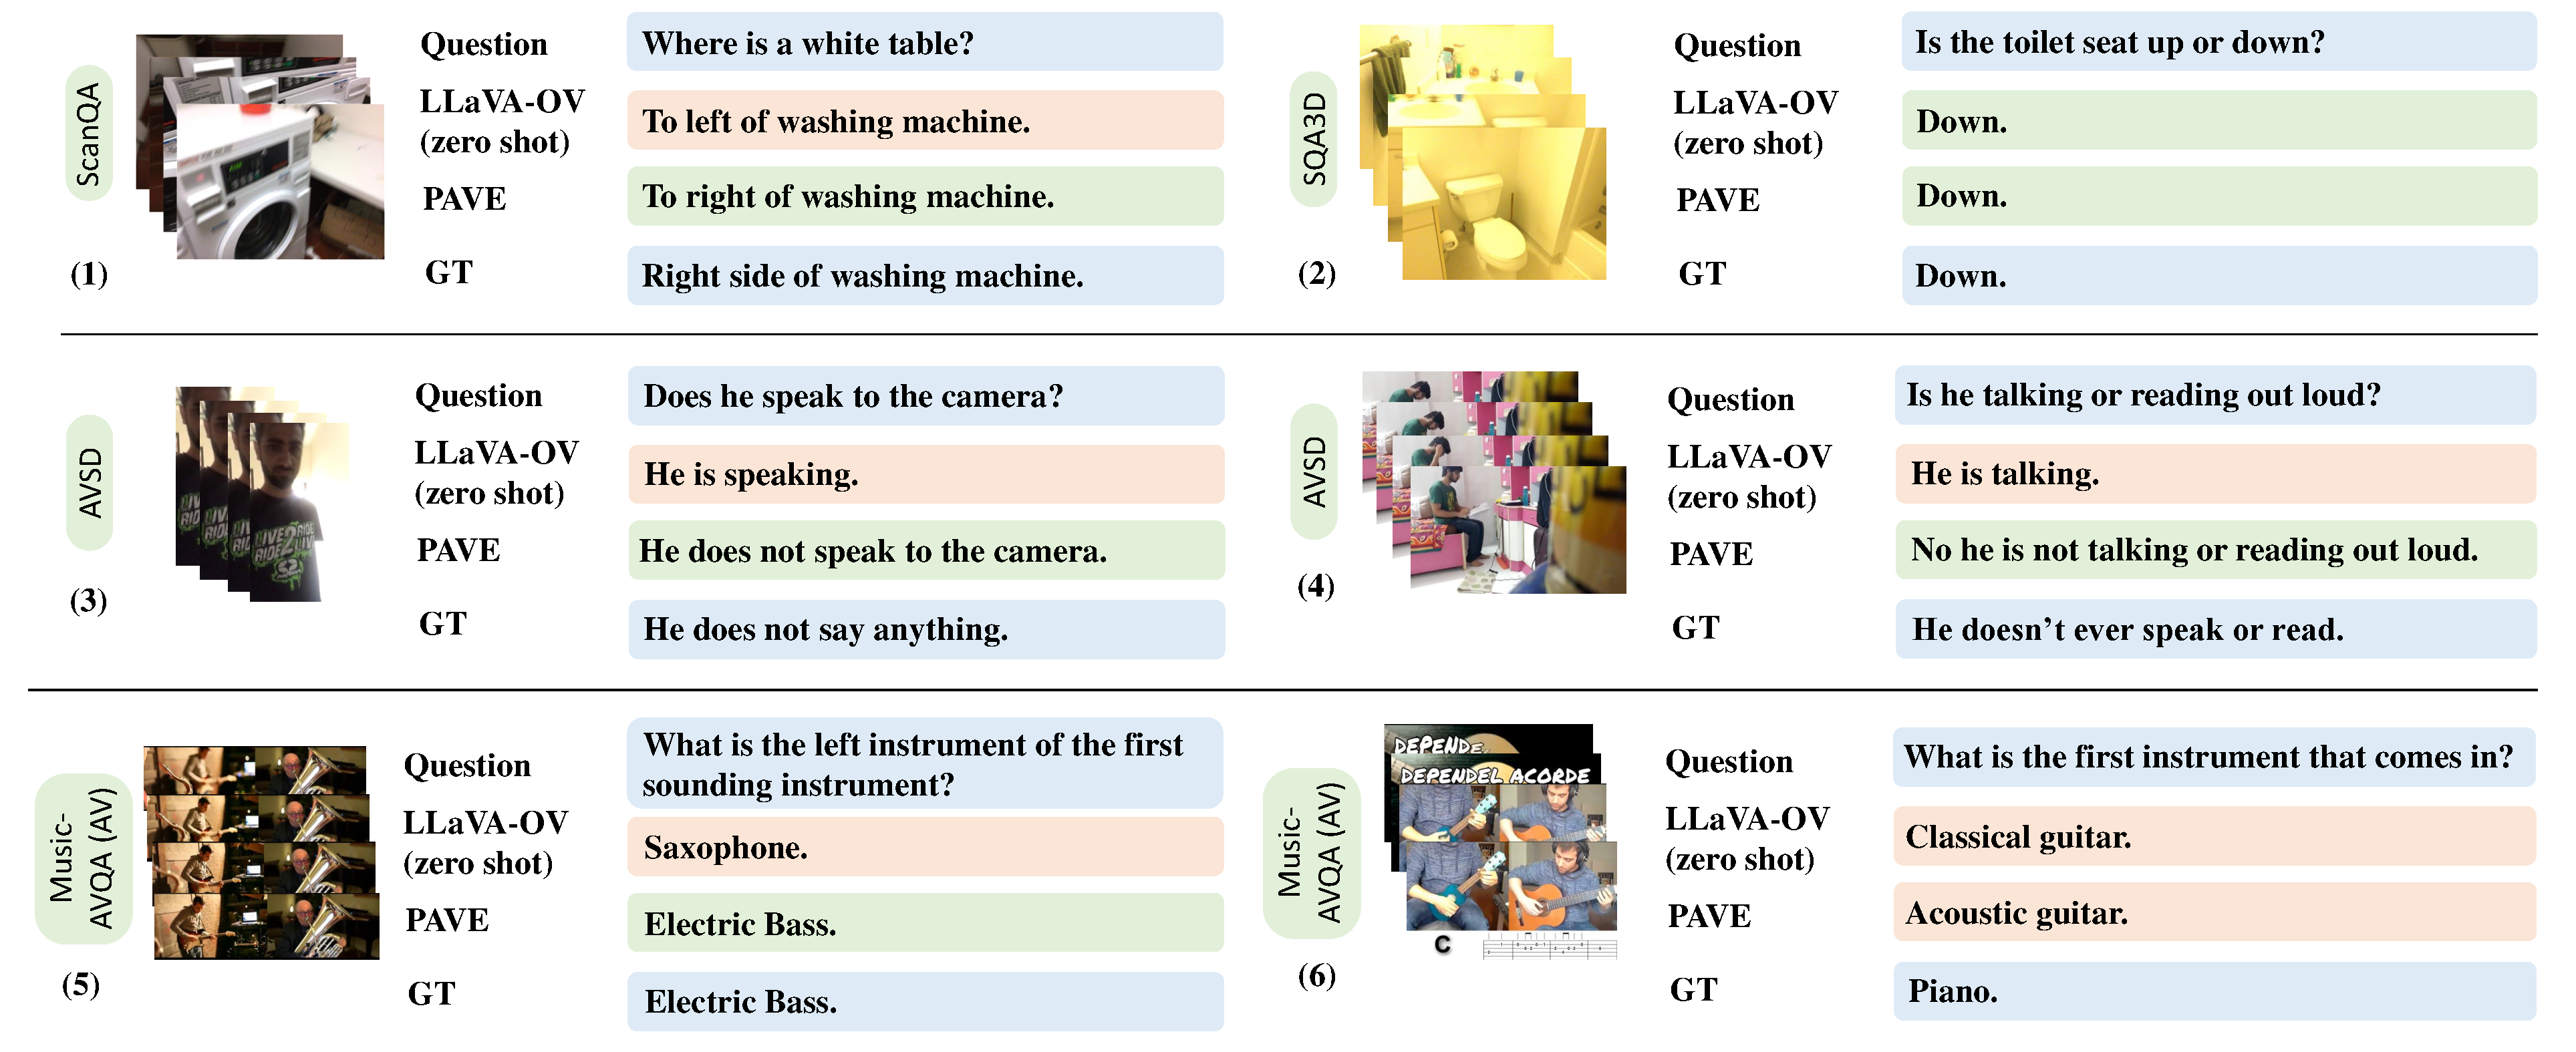
\includegraphics[width=0.92\linewidth]{figures/qa_visualization_updated2.pdf}
    \vspace{-1em}
    \caption{\textbf{Visualization of sample results}. We visualize the compare the results from our base model LLaVA-OneVision (under zero-shot inference) and PAVE across 3D QA and audio-visual QA tasks. Both succeful and failure cases are shown. 
    }
    %PAVE adapts LLaVA-OneVision to 3D QA and audio-visual tasks. The visualization provides the predictions from LLaVA-OneVision (zero-shot) and PAVE. PAVE learns to utilize 3D information and audio information for reasoning and thus improves the model performance. Specifically, in sample (6), when visual information conflicts with the audio information, the visual information will prevail given that PAVE is based on a Video LLM that is pre-trained on a visual-only dataset.}
    \label{fig:qa_visualization}
    \vspace{-0.5em}
\end{figure*}


\begin{figure*}[t!]
    \centering
    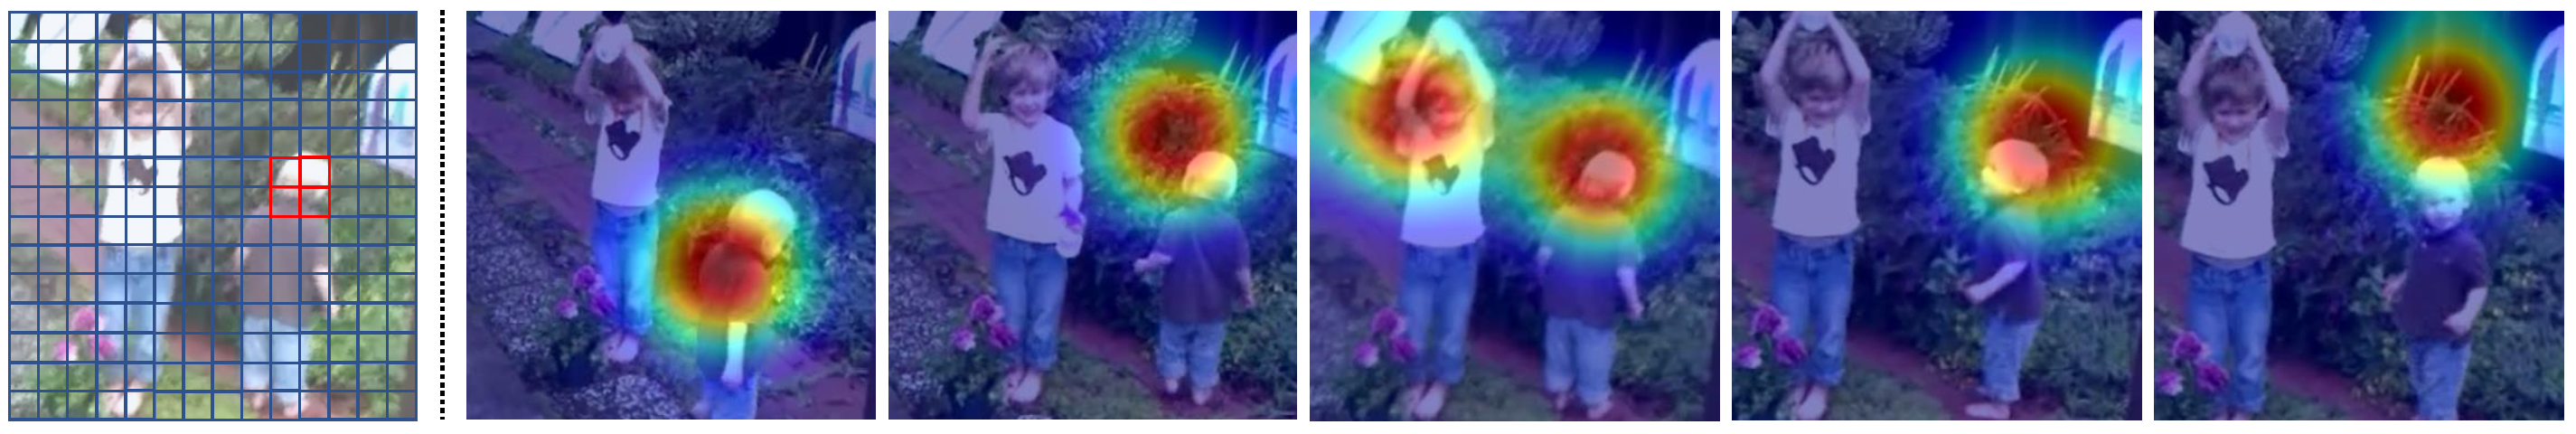
\includegraphics[width=0.90\linewidth]{figures/cross_attention_visualization.pdf}
    \vspace{-0.5em}
    \caption{\textbf{Visualization of cross-attention scores in PAVE} when injecting high frame rate videos as the side-channel. Cross-attention scores are calculated between the selected video tokens from the original low frame rate video (red cells on the left) and side-channel tokens from the high frame rate video. Scores are displayed as heatmaps over densely sampled video frames (on the right).} %This shows that cross-attention can effectively collect related information from densely sampled video frames.}
    \label{fig:cross_attention}
    \vspace{-1.5em}
\end{figure*}

\medskip
\noindent \textbf{Multi-task learning.} Moreover, we explore the potential of training multiple patches simultaneously and study the effects of such multi-task learning. We consider the setting of multiple tasks share overlapping side-channels (\eg, high-frame-rate video). In this case, multiple patches can be learned jointly, leading to potential enhancement across their corresponding side-channels.

As a first step to demonstrate this possibility, we design an experiment to integrate high frame rate video patch and audio-visual path for high frame rate audio-visual QA. Specifically, we build on the patch learned for injecting high frame rate videos (PAVE-7B model in Table~\ref{tab:general_video_understanding}), and train an additional patch for audio-visual QA on the AVSD training set. During training, the old patch is kept frozen and only the audio-visual patch is learned.  During the inference, we activate both patches, and PAVE takes input key frames (\ie low frame rate video), high frame rate video, and audio as input. Table~\ref{tab:avsd_with_dense_frames} shows that our multi-task learning leads to a notable improvement (\textit{+7.5} in CIDEr scores) on the AVSD test set, demonstrating the possibility and the benefit of training multiple patches together. We provide further discussion in Sec.\ \ref{sec:conclusion}.

%There are two distinct scenarios in multi-task joint training: 1. If individual tasks (e.g., audio-visual and 3D) do not share overlapping modalities, joint training is effectively equivalent to training each task independently. In this case, only the task-relevant patch is used for each sample. 2. When multiple tasks share overlapping modalities (e.g., high-frame-rate video) beyond raw video, multiple patches are utilized during training, leading to a more comprehensive understanding of the video and potential improvement in performance.

%We conduct additional experiments to demonstrate modality enhancement. Specifically, we use the enhanced video understanding patch (PAVE-7B model in Table~\ref{tab:general_video_understanding}) and train a new patch for audio-visual QA on the AVSD training set with the enhanced video understanding patch frozen. During the inference, we activate both patches, and PAVE takes input key frames, high framerate video, and audio as input. Table~\ref{tab:avsd_with_dense_frames} shows multi-task joint training results in a notable improvement (\textbf{+7.5}) on the AVSD test set, demonstrating the possibility and the benefit of training multiple patches together. We provide further discussion in the Appendix about leveraging multiple patches at the same time.

% Yin: The text was very redundant. DO NOT REPEAT THE TEXT IN THE PAPER.

\medskip
\noindent\textbf{Results visualization and diagnosis.} 
Finally, we visualize sample results of 3D QA and audio-visual QA in Figure~\ref{fig:qa_visualization}. An interesting failure case of PAVE, as we previously mentioned in Sec.\ \ref{section_res_audio} is shown in sample (6), where the piano is present in the audio but never appears visually in the video, creating a conflict between the auditory and visual information. In this case, PAVE produces inaccurate answers.

To further diagnose our model, we visualize cross-attention scores between video tokens and side-channel tokes in PAVE's fusion function. Figure~\ref{fig:cross_attention} shows  heatmaps of cross-attention scores when injecting high high frame rate videos as the side-channel (corresponding to results of PAVE-7B in Table~\ref{tab:general_video_understanding}). We calculate the cross-attention scores between the selected video tokens (shown in the red cells) from the original low frame rate videos, and the side-channel tokens from the high frame rate videos. The visualization shows that the peaks of the heatmap keep track of visually similar regions in densely sampled video frames. This result indicates that the fusion function in PAVE facilitates explicit alignment between video tokens and side-channel tokens, and thus allows for effectively integrating information from the side-channel.

%the heatmap has the highest response on the regions that contain a similar visual concept as the one represented by selected tokens from $\mathbf{z}^v$. 



%Figure~\ref{fig:qa_visualization} further visualizes results of 3D and audio-visual QA. 

%For 3D QA, PAVE adapts LLaVA-OneVision by incorporating additional spatial information, enabling the model to understand the relative positions of objects within the scene. 
%In the audio-video setting, PAVE enhances Video LLM's reasoning capabilities by incorporating audio input, thereby improving the model's performance and mitigating hallucination in audio-visual scenarios.
%Specifically, we visualize samples from the audio-visual split of Music-AVQA in (5) and (6). For sample (6) in Figure~\ref{fig:qa_visualization}, the piano is present in the audio but never appears visually in the video, creating a conflict between the auditory and visual information. In this case, PAVE produces inaccurate responses.
%We hypothesize that since the Video LLM that PAVE adapted is trained on visual-only data, the visual information has a higher influence than audio, which ultimately skews the prediction.


%\medskip
%\noindent\textbf{Visualization of cross-attention in PAVE.} 
%Figure~\ref{fig:cross_attention} visualizes the cross-attention map in enhanced video QA. In this setting, we use the densely sampled video frames as the side-channel information. We calculate the cross-attention activation values between the selected tokens (shown in the red cells) from the Video LLM visual encoder $\mathbf{z}^v$, and the tokens from the side-channel $\mathbf{z}^s$. The visualization indicates that the heatmap has the highest response on the regions that contain a similar visual concept as the one represented by selected tokens from $\mathbf{z}^v$. This indicates the cross-attention module captures the similarity of the visual concept between $\mathbf{z}^v$ and $\mathbf{z}^s$ and thus enables PAVE to effectively collect information from the side-channel.



%